\documentclass[aspectratio=169]{beamer} %% for 16:9 use this line
%%\documentclass{beamer}  %% For 4:3 ratio use this line
\usepackage[utf8]{inputenc}
\usepackage[T1]{fontenc}
\usepackage{lipsum} 
\usepackage{bm}
\usepackage{graphicx}
\usepackage{animate}
\usepackage{subcaption}
% import citation package
\usepackage[backend=biber, style=authoryear]{biblatex}
\addbibresource{./biblio.bib}
\AtBeginBibliography{\small}

% footnote without number
\newcommand\blfootnote[1]{
\begingroup
\renewcommand\thefootnote{}\footnote{#1}
\addtocounter{footnote}{-1}
\endgroup
}

\usetheme{CEA2023}
\setlength{\columnsep}{0.05cm}
\title[Data Assimilation for Meshless Simulation]  %optional
{Ensemble Data Assimilation Method Applied to Meshless Simulations}
% \subtitle{Using the CEA beamer template}
\date[06-03-2024]  %optional
{June the 3\textsuperscript{rd} 2024}
\author[M. Duvillard]  %optionam
{Marius Duvillard \inst{1} \texttt{(\small marius.duvillard\myat cea.fr)} \\
Olivier Le Maître \inst{2} \inst{3} \texttt{(\small olivier.le-maitre \myat polytechnique.edu)}}

\institute[short-inst]{
  \inst{1} CEA DES/IRESNE/DEC/SESC Cadarache 
  \inst{2} Centre de Mathématiques Appliquées, Ecole Polytechnique 
  \inst{3} CNRS, Inria
}

% uncomment the following lines if you do not want dedicated outlines before
% each section
\AtBeginSection{}

% use your thanks-message in the last frame
\setvalue{\ThxMessage}{Thanks! Any questions?}
% Change the logo 
\titlegraphic{logos/IRESNE_redred.png}

% introduce another logo for a second author or affiliation
% secondlogo applies to the first page only
% \setvalue{\secondlogo}{MyLogo.png}

\begin{document}

% info: the plain removes the footline from the titlepage; noframenumbering
% neglects it from the total count of the slides
\begin{frame}[decorated] %Decorated bring the logo and corner
    \titlepage
\end{frame}

\begin{frame}[righttransition]{Outline}  % or Table of Contents
    \tableofcontents
\end{frame}

\section{Introduction and Background}
\subsection{Data assimilation}
\begin{frame}{Data assimilation}
    \begin{Definition}
        Data assimilation is an \textcolor{macaron}{analysis} that combines, in some optimal fashion, the time-distributed \textcolor{yellow}{observations} with the \textcolor{darkblue}{dynamic model}, tacking into account the \textcolor{darkblue}{background} (prior) information to approximate the true state of some physical system through time~\cite{asch_data_2016}.
    \end{Definition}
    \begin{figure}
        \centering
        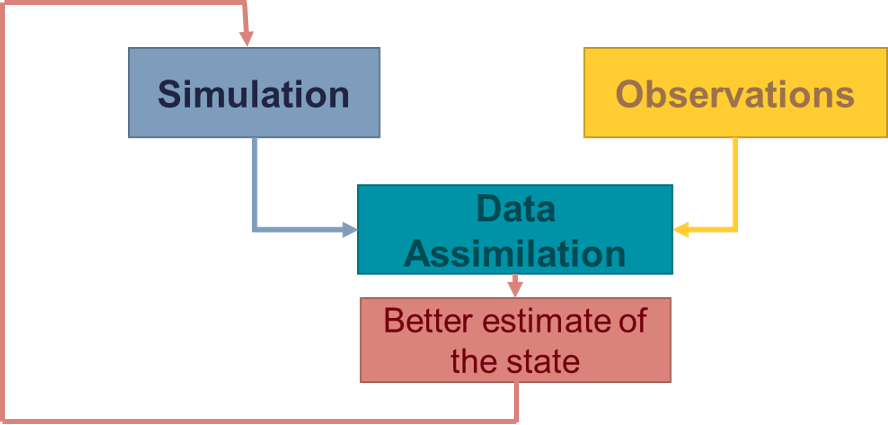
\includegraphics[width=0.5\textwidth]{images/data_assimilation_scheme.png}
    \end{figure}
    \hfill
\end{frame}

\begin{frame}{Data assimilation}{Notation and formulation}
    \small
    We note $X_k$ the state, $Y_k$ the observation at discrete time step $k$
    \begin{block}{Sequential Filtering}
        Update the state $X_{k+1}$ given a predicted state $X_{k+1}$
        and the current observation $y_{k+1}$ based on Bayesian estimation --> *posterior distribution*: $p(X_{k+1} \mid Y_{k+1}) \propto p(Y_{k+1} \mid X_{k+1}) p(X_{k+1})$
    \end{block}
    \vfill
    \begin{columns}
        \begin{column}{0.5\textwidth}
            \textbf{Hidden Markov Chain Model}
            \begin{itemize}
                \item \textbf{Initial condition}: $X_0 \sim \mathcal N(x_0, P_0)$
                \item \textcolor{darkblue}{\textbf{Model forecast with error}}:
                      $X_{k+1} = \mathcal M(X_k) + \eta_{k+1},\quad \eta_{k+1} \sim \mathcal N(0, P_{k+1})$
                \item \textcolor{yellow}{\textbf{Observation equation with error}}:
                      $Y_{k+1} = \mathcal H(X_{k+1}) + \eta_{k+1},\quad \varepsilon_{k+1} \sim \mathcal N(0, R_{k+1})$
                \item $X_0 \perp \eta_{k+1} \perp \varepsilon_{k+1}$
            \end{itemize}
        \end{column}
        \begin{column}{0.5\textwidth}
            \begin{figure}
                \centering
                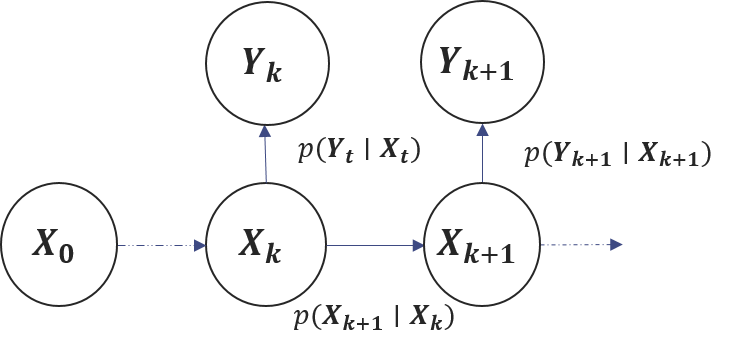
\includegraphics[width=0.8\textwidth]{images/markov_chain.png}
            \end{figure}
        \end{column}
    \end{columns}
\end{frame}

\subsubsection{Sequential Filtering - Ensemble Kalman Filter}
\begin{frame}{Sequential Filtering - Ensemble Kalman Filter}
    \begin{exampleblock}{}
        \begin{itemize}
            \item Generalization of the \textbf{Kalman Filter} where the state distribution is represented by an \textbf{ensemble} of state in order to estimate statistics and propagate uncertainty~\cite{evensen_sequential_1994}.
            \item Adapted to \textbf{non-linear} and \textbf{high-dimansional} state.
        \end{itemize}
    \end{exampleblock}
    \begin{columns}
        \begin{column}{0.6\textwidth}
            \begin{itemize}
                \item<1-> \textbf{Initialization} \\
                    Sample $N$ states $\left\{x^i_0\right\}_{i=1}^N \stackrel{iid}{\sim} X_0$
                \item<2-> \textbf{Forecast} (with numerical simulation code) \\
                    $\hat x^i_{k+1} = \mathcal M(x_{k}^i), \quad i = 1, \dots, N$
                \item<3-> \textbf{Measurement and prediction}
                    measure $y_{k+1}$, prediction $h^i_{k+1} = \mathcal (\hat x_{k+1}^i) \quad i = 1, \dots, N$

                \item<4-> \textbf{Analysis} \footnotemark[1] A weighted linear combination of $\hat x_{k+1}^i$ \\
                    $x^i_{k+1} = \hat x^i_{k+1} + \sum_{j=1}^N \bm F_{ij} \hat x^i_{k+1}$, \\ where $\bm F$ depends on $\left(y_{k+1}, \left\{h^i_{k+1}\right\}_{i=1}^N\right)$
            \end{itemize}
        \end{column}
        \begin{column}{0.4\textwidth}
            \begin{figure}
                \centering
                \only<1>{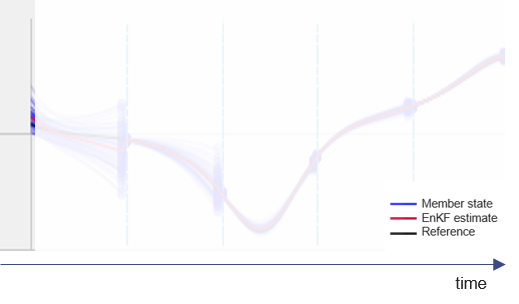
\includegraphics[width=\textwidth]{images/initialization.png}}
                \only<2>{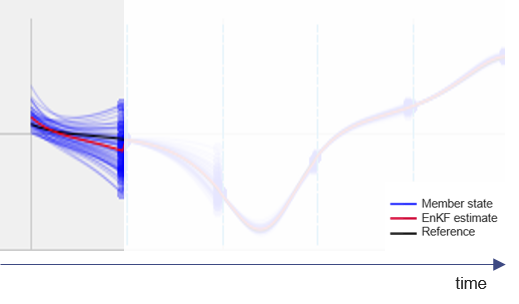
\includegraphics[width=\textwidth]{images/propagation.png}}
                \only<3>{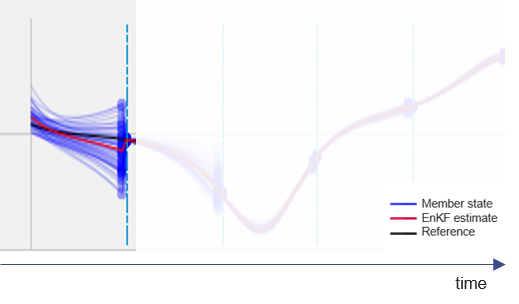
\includegraphics[width=\textwidth]{images/obs_analasis.png}}
                \only<4>{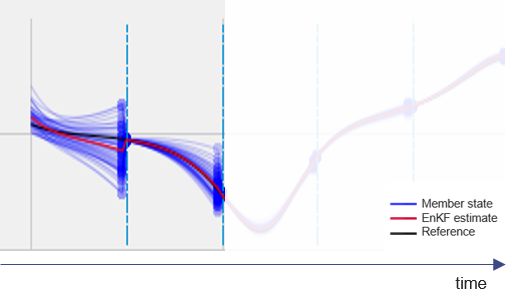
\includegraphics[width=\textwidth]{images/obs_analasis2.png}}
                \only<5>{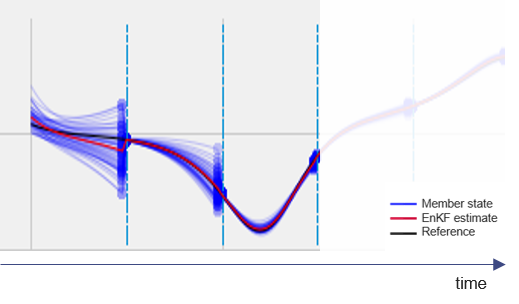
\includegraphics[width=\textwidth]{images/obs_analasis3.png}}
                \only<6>{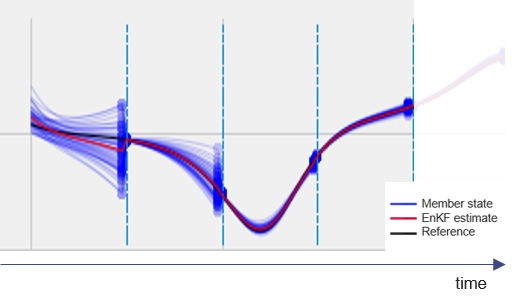
\includegraphics[width=\textwidth]{images/obs_analasis4.png}}
                \only<7>{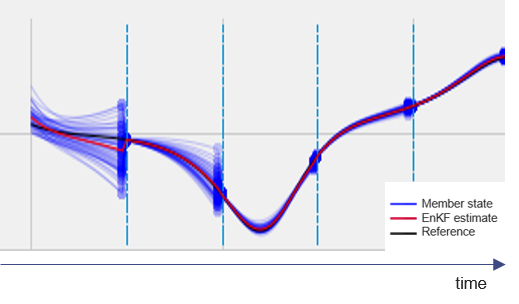
\includegraphics[width=\textwidth]{images/obs_analasis5.png}}
            \end{figure}
        \end{column}
    \end{columns}
    \footnotetext[1]{\tiny equivalent formulation of the original formulation see~\cite{siripatana_combining_2019}}
\end{frame}

\subsection{Meshless simulation}
\begin{frame}{Meshless simulation}
    \small
    \begin{columns}
        \begin{column}{0.5\textwidth}
            \begin{Definition}
                Meshfree methods are class of method that relies on the discretize the solution thanks to particles that move according to the velocity field. \\
                = \textbf{Lagrangian method}
            \end{Definition}

            Particles are defined with a position $\bm z_p$, an intensity $\Gamma_p$ and a kernel $\phi_h$

            Let $\omega$ a scalar field discretize with a set of particle $Z = \left\{z_p, \Gamma_p\right\}_{p=1}^{N_p}$:
            \begin{equation*}
                \omega (z) = \sum_{i=1}^{N_p} \Gamma_p \phi_h(z - z_p)
            \end{equation*}
        \end{column}
        \begin{column}{0.5\textwidth}

            \begin{figure}
                \centering
                \begin{subfigure}[t]{\textwidth}
                    \centering
                    \animategraphics[loop, autoplay, width=0.45\textwidth]{10}{images/lag_representation/b1da922d43984958b92c8b71e90b82a600e60cucwjbaqV5A-}{0}{35}
                    \caption{Lagrangian representation}
                \end{subfigure}
                \vfill
                \begin{subfigure}[b]{\textwidth}
                    \centering
                    \animategraphics[loop, autoplay, width=0.45\textwidth]{10}{images/euler_representation/75da49fc4fc047fdc8e7e2e69d8d6aca0GH5HJHxDWrygBfE-}{0}{35}
                    \caption{Eulerian representation}
                \end{subfigure}
            \end{figure}
        \end{column}
    \end{columns}

\end{frame}

\section{Intensity correction}

\begin{frame}{Intensity correction}
    We adapt the EnKF filter for this type of simulation.
    $\left\{z_p, \Gamma_p\right\}_{p=1}^{N_p} -> ?$

    \begin{block}{EnKF correction}
        test
    \end{block}
    %     \begin{block}<1->{First case: same particles positions}
    %         test
    %     \end{block}
    %     \begin{block}<2->{General case: Different particles configurations}
    %         test
    %     \end{block}
\end{frame}

% \begin{frame}{Part EnKF}
%     \subtitle{Project solution on each forecast configuration}
% \end{frame}

% \begin{frame}{Remesh EnKF}
%     \subtitle{Regrid on a common particle configuration}
% \end{frame}

% \section{Position update}
% \begin{frame}{Intensity correction - limitation}
% \begin{columns}
%     \begin{column}{0.5\textwidth}
%         \textbf{Double-penalty error}
%         Overpenalization of model and observation errors
%         \begin{figure}
%             \centering
%             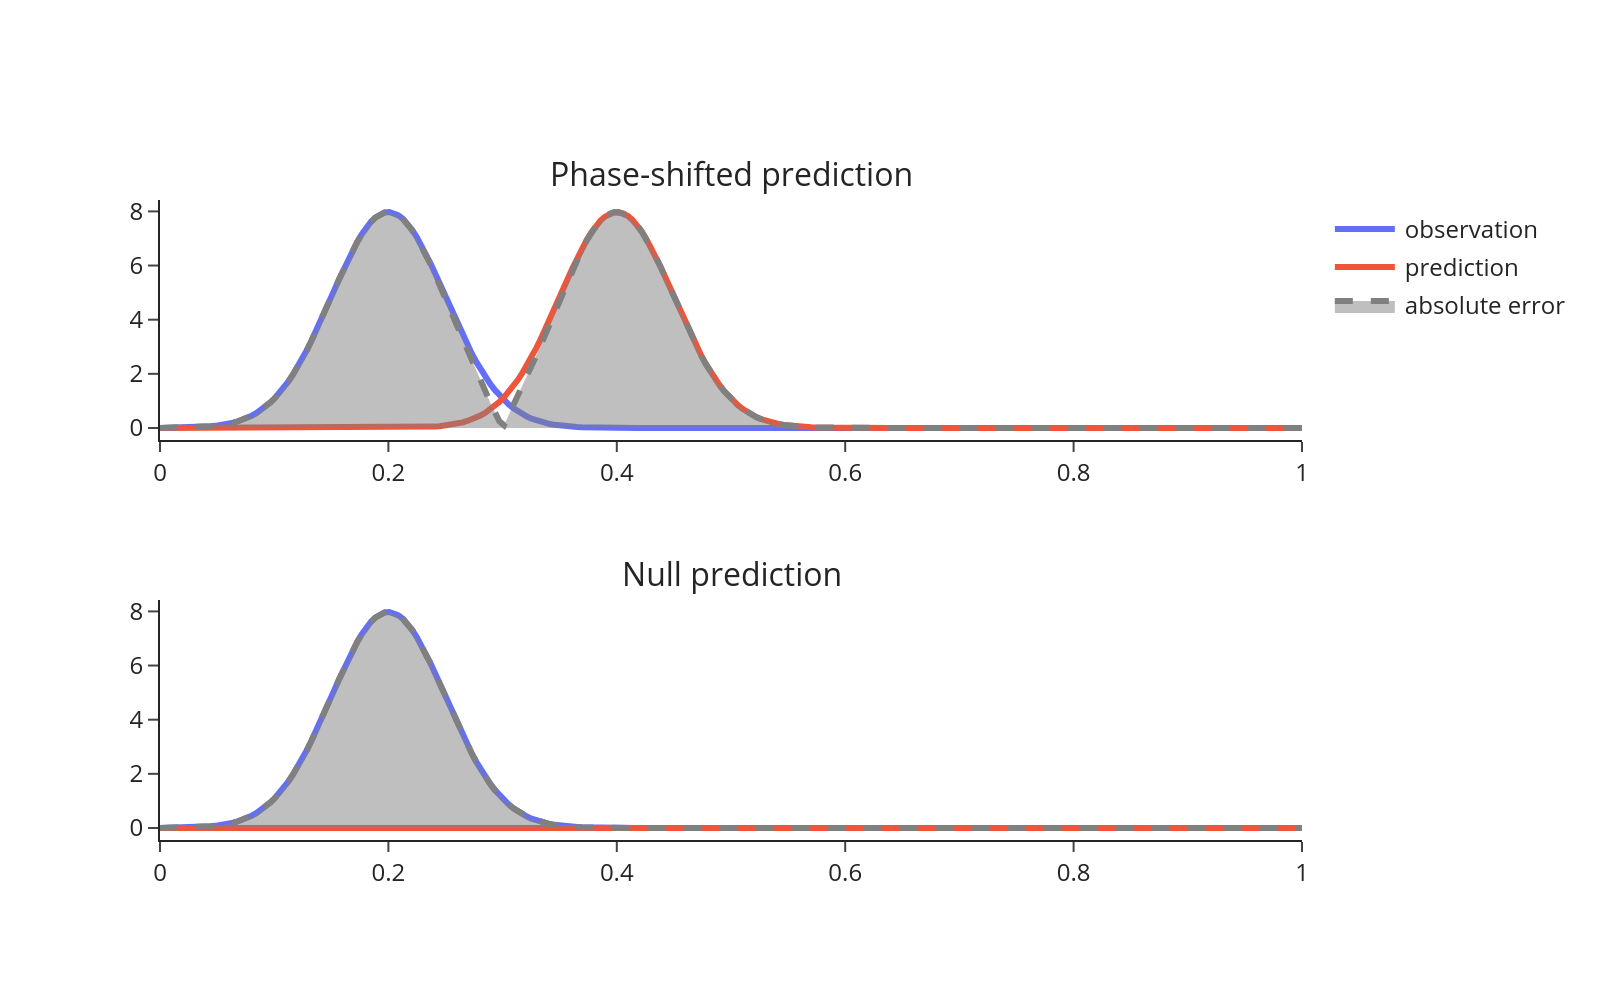
\includegraphics[width=0.8\textwidth]{images/double_penalisation.png}
%         \end{figure}
%     \end{column}

%     \begin{column}{0.5\textwidth}
%         \textbf{Confined to the particle support}
%         \begin{itemize}
%             \item Previous filter only update intensities
%                   %   \begin{equation*}
%                   %       \{\bm x_i \Gamma^f\} \mapsto \{\bm x_i \Gamma^a\}
%                   %   \end{equation*}
%             \item Particles might be unadequat to the analysis solution
%                   \begin{figure}
%                       \centering
%                       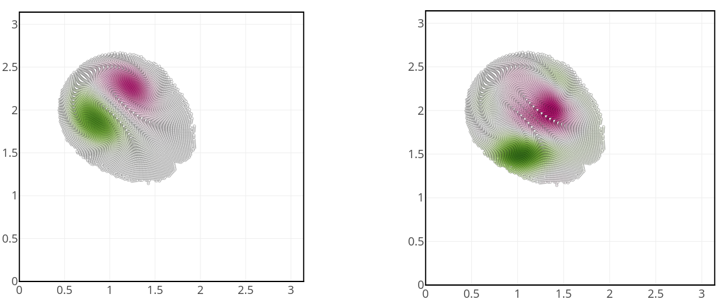
\includegraphics{images/unalign_discretization.png}
%                   \end{figure}
%         \end{itemize}
%     \end{column}
% \end{columns}
% test...
% \end{frame}

% \begin{frame}{Position correction}
%     \begin{block}{Hypothesis}
%         Error in the velocity field lead to error in the integration of the particles position.
%     \end{block}
%     \begin{block}{Goal}
%         Correct the position by integrating a velocity field.
%     \end{block}

%     % \begin{equation*}
%     %     \Phi(x)
%     % \end{equation*}
% \end{frame}

\closingframe


\begin{frame}[allowframebreaks, noframenumbering]
    \frametitle{References}
    \printbibliography % Print the bibliography
\end{frame}

% \section*{Addendum}
% \begin{frame}{EnKF update}
%     \emph{Be successful with your presentation!}
% \end{frame}

\end{document}
